%% PÁGINA DE ROSTO
\begin{titlepage}
\begin{center}%{\large \sc Title in english}
\par
\vspace{90pt}
{\large \sc BIZ0433 - Inferência Filogenética: Filosofia, Método e Aplicações.}\par
\par
\vspace{90pt}
{\LARGE Tutoriais}\par
\vspace{10pt}
{\LARGE Prática e Teoria em Cladística Computacional}\par
\vspace{25pt}
\end{center}\par
\vspace{120pt}
\hspace*{40pt}\parbox{15cm}{{\textbf{Responsável:} Prof. Fernando P. de L. Marques (\href{mailto:fernando@ib.usp.br}{fernando@ib.usp.br})\\Departamento de Zoologia\\Instituto de Biociências\\Universidade de São Paulo\\ Rua do Matão, tv. 14, no. 101 - Cidade Universitária\\ 05508-090 - São Paulo - Brasil}}\par
\par\vfill\begin{center}
\textbf{{\large São Paulo}}\\
Versão de \large \today\\
%%%%%%%%%%%%%%%%%%%%%%%%%%% FIGURA DO FILE SYSTEM %%%%%%%%%%%%%%%%%%%%%%%%%%%
%  \vspace{-1em}
  \begin{figure}[H]
    %\ffigbox[\FBwidth]
      {\includegraphics[scale=0.6]{figures/by-sa.eps}}
      %{\caption[\textit{Lunux File System}]{Estrutura hierárquica do \textit{file system} do Linux.}\label{tut1:fig:fs}}
  \end{figure}

%%%%%%%%%%%%%%%%%%%%%%%%%%% FIM DA FIGURA DO FILE SYSTEM %%%%%%%%%%%%%%%%%%%%%%%%%%%
{\small Estes tutoriais estão licenciados sob a\\
\href{http://creativecommons.org/licenses/by-sa/4.0/}{Creative Commons Attribution-ShareAlike 4.0 International License}}
\end{center}\end{titlepage}

\pagestyle{empty} % Limpa o cabeçalho definido no meta.tex
\pagenumbering{roman} % Números das páginas em romanos

% ÍNDICE
\dominitoc % for table of contents within the chapter
\tableofcontents
% LISTA DE TABELAS
\listoftables

% LISTA DE FIGURAS
\listoffigures
